%%%%%%%%%%%%%%%%%%%%%%%%%%%%%%%%%%%%%%%%%%%%%%%%%%%%%%%%%%%%%%%%%%%%%%%%%%%%%%%%
%% Plantilla de memoria en LaTeX para la EIF - Universidad Rey Juan Carlos
%%
%% Por Gregorio Robles <grex arroba gsyc.urjc.es>
%%     Grupo de Sistemas y Comunicaciones
%%     Escuela de Ingeniería de Fuenlabrada
%%     Universidad Rey Juan Carlos
%% (muchas ideas tomadas de Internet, colegas del GSyC, antiguos alumnos...
%%  etc. Muchas gracias a todos)
%%
%% La última versión de esta plantilla está siempre disponible en:
%%     https://github.com/gregoriorobles/plantilla-memoria
%%
%% Para obtener PDF, ejecuta en la shell:
%%   make
%% (las imágenes deben ir en PNG o JPG)

%%%%%%%%%%%%%%%%%%%%%%%%%%%%%%%%%%%%%%%%%%%%%%%%%%%%%%%%%%%%%%%%%%%%%%%%%%%%%%%%

\documentclass[a4paper, 12pt]{book}
%\usepackage[T1]{fontenc}

\usepackage[a4paper, left=2.5cm, right=2.5cm, top=3cm, bottom=3cm]{geometry}
\usepackage{times}
\usepackage[utf8]{inputenc}
\usepackage[spanish]{babel} % Comenta esta línea si tu memoria es en inglés
\usepackage{url}
%\usepackage[dvipdfm]{graphicx}
\usepackage{graphicx}
\usepackage{float}  %% H para posicionar figuras
\usepackage[nottoc, notlot, notlof, notindex]{tocbibind} %% Opciones de índice
\usepackage{latexsym}  %% Logo LaTeX

\title{Memoria del Proyecto}
\author{Nombre del autor}

\renewcommand{\baselinestretch}{1.5}  %% Interlineado

\begin{document}
	
	\renewcommand{\refname}{Bibliografía}  %% Renombrando
	\renewcommand{\appendixname}{Apéndice}
	
	
	%%%%%%%%%%%%%%%%%%%%%%%%%%%%%%%%%%%%%%%%%%%%%%%%%%%%%%%%%%%%%%%%%%%%%%%%%%%%%%%%
	% PORTADA
	
	\begin{titlepage}
		\begin{center}
			\includegraphics[scale=0.6]{img/URJ_logo_Color_POS.png}
			
			\vspace{1.75cm}
			
			\LARGE
			ESCUELA DE INGENIERÍA DE FUENLABRADA
			\vspace{1cm}
			
			\LARGE
			GRADO EN INGENIERIA EN TECNOLOGIAS DE LA TELECOMUNICACION
			
			\vspace{1cm}
			\LARGE
			\textbf{TRABAJO FIN DE GRADO}
			
			\vspace{1cm}
			
			\Large
			CONFIGURACIÓN Y PRUEBAS DE UN PLANO DE CONTROL IN-BAND SDN/OPENFLOW: MAQUETA CON SWITCHES ETHERNET  
			
			\vspace{2cm}
			
			\large
			Autor : Luis Haro Peña \\
			Tutor : Pedro de las Heras Quirós\\
			Cotutor: Eva María Castro Barbero
			\vspace{1cm}
			
			\large
			Curso académico 2022/2023
			
		\end{center}
	\end{titlepage}
	
	\newpage
	\mbox{}
	\thispagestyle{empty} % para que no se numere esta pagina
	
	
	
	%%%%%%%%%%%%%%%%%%%%%%%%%%%%%%%%%%%%%%%%%%%%%%%%%%%%%%%%%%%%%%%%%%%%%%%%%%%%%%%%
	%%%% Para firmar
	\clearpage
	\pagenumbering{gobble}
	\chapter*{}
	
	\vspace{-4cm}
	\begin{center}
		\LARGE
		\textbf{Trabajo Fin de Grado/Máster}
		
		\vspace{1cm}
		\large
		Configuración y Pruebas de un Plano de Control In-Band SDN/Openflow: Maqueta con Switches Ethernet
		
		\vspace{1cm}
		\large
		\textbf{Autor :} Luis Haro Peña \\
		\textbf{Tutor :} Pedro de las Heras Quirós
		
	\end{center}
	
	\vspace{1cm}
	La defensa del presente Proyecto Fin de Carrera se realizó el día \qquad$\;\,$ de \qquad\qquad\qquad\qquad \newline de 2023, siendo calificada por el siguiente tribunal:
	
	
	\vspace{0.5cm}
	\textbf{Presidente:}
	
	\vspace{1.2cm}
	\textbf{Secretario:}
	
	\vspace{1.2cm}
	\textbf{Vocal:}
	
	
	\vspace{1.2cm}
	y habiendo obtenido la siguiente calificación:
	
	\vspace{1cm}
	\textbf{Calificación:}
	
	
	\vspace{1cm}
	\begin{flushright}
		Fuenlabrada, a \qquad$\;\,$ de \qquad\qquad\qquad\qquad de 2023
	\end{flushright}
	
	%%%%%%%%%%%%%%%%%%%%%%%%%%%%%%%%%%%%%%%%%%%%%%%%%%%%%%%%%%%%%%%%%%%%%%%%%%%%%%%%
	%%%% Dedicatoria
	
	\chapter*{}
	\pagenumbering{Roman} % para comenzar la numeracion de paginas en numeros romanos
	\begin{flushright}
		\textit{Dedicado a todos los que me han apoyado con este trabajo, y sobretodo, a los que ya no están.}
	\end{flushright}
	
	%%%%%%%%%%%%%%%%%%%%%%%%%%%%%%%%%%%%%%%%%%%%%%%%%%%%%%%%%%%%%%%%%%%%%%%%%%%%%%%%
	%%%% Agradecimientos
	
	\chapter*{Agradecimientos}
	%\addcontentsline{toc}{chapter}{Agradecimientos} % si queremos que aparezca en el índice
	\markboth{AGRADECIMIENTOS}{AGRADECIMIENTOS} % encabezado 
	
	Estimada familia, pareja, amigos y seres queridos,
	
	Hoy quiero tomar un momento para expresar mi más profundo agradecimiento por todo su apoyo y amor incondicional durante mi trayectoria académica y, en particular, en la culminación de mi trabajo de fin de grado. Vuestra presencia constante, aliento y comprensión han sido fundamentales en mi camino hacia el éxito.
	
	En primer lugar, quiero agradecer a mis padres, quienes me han brindado un apoyo inquebrantable desde el principio. Vuestra dedicación, paciencia y sacrificios han sido el pilar sobre el cual he construido mi educación. Gracias por estar siempre ahí, incluso en los momentos más difíciles.
		
	A mi pareja, quiero expresar mi más profundo agradecimiento por tu amor, paciencia y apoyo a lo largo de este viaje académico. Tú has sido mi roca, mi fuente de inspiración y mi motivación constante. Tus palabras de aliento y tu presencia reconfortante me han dado fuerzas para superar cualquier obstáculo que se haya presentado en el camino. Gracias por ser mi compañera de vida y por estar a mi lado en cada paso del camino.
	
	Con gratitud,
	Luis.
	
	%%%%%%%%%%%%%%%%%%%%%%%%%%%%%%%%%%%%%%%%%%%%%%%%%%%%%%%%%%%%%%%%%%%%%%%%%%%%%%%%
	%%%% Resumen
	
	\chapter*{Resumen}
	%\addcontentsline{toc}{chapter}{Resumen} % si queremos que aparezca en el índice
	\markboth{RESUMEN}{RESUMEN} % encabezado
	
	Aquí viene un resumen del proyecto.
	Ha de constar de tres o cuatro párrafos, donde se presente de manera clara y concisa de qué va el proyecto. 
	Han de quedar respondidas las siguientes preguntas:
	
	\begin{itemize}
		\item ¿De qué va este proyecto? ¿Cuál es su objetivo principal?
		\item ¿Cómo se ha realizado? ¿Qué tecnologías están involucradas?
		\item ¿En qué contexto se ha realizado el proyecto? ¿Es un proyecto dentro de un marco general?
	\end{itemize}
	
	Lo mejor es escribir el resumen al final.
	
	%%%%%%%%%%%%%%%%%%%%%%%%%%%%%%%%%%%%%%%%%%%%%%%%%%%%%%%%%%%%%%%%%%%%%%%%%%%%%%%%
	%%%% Resumen en inglés
	
	\chapter*{Summary}
	%\addcontentsline{toc}{chapter}{Summary} % si queremos que aparezca en el índice
	\markboth{SUMMARY}{SUMMARY} % encabezado
	
	Here comes a translation of the ``Resumen'' into English. 
	Please, double check it for correct grammar and spelling.
	As it is the translation of the ``Resumen'', which is supposed to be written at the end, this as well should be filled out just before submitting.
	
	
	%%%%%%%%%%%%%%%%%%%%%%%%%%%%%%%%%%%%%%%%%%%%%%%%%%%%%%%%%%%%%%%%%%%%%%%%%%%%%%%%
	%%%%%%%%%%%%%%%%%%%%%%%%%%%%%%%%%%%%%%%%%%%%%%%%%%%%%%%%%%%%%%%%%%%%%%%%%%%%%%%%
	% ÍNDICES %
	%%%%%%%%%%%%%%%%%%%%%%%%%%%%%%%%%%%%%%%%%%%%%%%%%%%%%%%%%%%%%%%%%%%%%%%%%%%%%%%%
	
	% Las buenas noticias es que los índices se generan automáticamente.
	% Lo único que tienes que hacer es elegir cuáles quieren que se generen,
	% y comentar/descomentar esa instrucción de LaTeX.
	
	%%%% Índice de contenidos
	\tableofcontents 
	%%%% Índice de figuras
	\cleardoublepage
	%\addcontentsline{toc}{chapter}{Lista de figuras} % para que aparezca en el indice de contenidos
	\listoffigures % indice de figuras
	%%%% Índice de tablas
	%\cleardoublepage
	%\addcontentsline{toc}{chapter}{Lista de tablas} % para que aparezca en el indice de contenidos
	%\listoftables % indice de tablas
	
	
	%%%%%%%%%%%%%%%%%%%%%%%%%%%%%%%%%%%%%%%%%%%%%%%%%%%%%%%%%%%%%%%%%%%%%%%%%%%%%%%%
	%%%%%%%%%%%%%%%%%%%%%%%%%%%%%%%%%%%%%%%%%%%%%%%%%%%%%%%%%%%%%%%%%%%%%%%%%%%%%%%%
	% INTRODUCCIÓN %
	%%%%%%%%%%%%%%%%%%%%%%%%%%%%%%%%%%%%%%%%%%%%%%%%%%%%%%%%%%%%%%%%%%%%%%%%%%%%%%%%
	
	\cleardoublepage
	\chapter{Introducción}
	\label{sec:intro} % etiqueta para poder referenciar luego en el texto con ~\ref{sec:intro}
	\pagenumbering{arabic} % para empezar la numeración de página con números
	
	
	
	
	\section{Sección}
	\label{sec:seccion}
	
	Este trabajo consiste en el análisis y comprensión de un plano de control In-Band SDN/Openflow en varios escenarios con diferente número de controladores.
	
	\subsection{Estilo}
	\label{subsec:estilo}
	
	TO DO
	
	
	%%%%%%%%%%%%%%%%%%%%%%%%%%%%%%%%%%%%%%%%%%%%%%%%%%%%%%%%%%%%%%%%%%%%%%%%%%%%%%%%
	%%%%%%%%%%%%%%%%%%%%%%%%%%%%%%%%%%%%%%%%%%%%%%%%%%%%%%%%%%%%%%%%%%%%%%%%%%%%%%%%
	% OBJETIVOS %
	%%%%%%%%%%%%%%%%%%%%%%%%%%%%%%%%%%%%%%%%%%%%%%%%%%%%%%%%%%%%%%%%%%%%%%%%%%%%%%%%
	
	\cleardoublepage % empezamos en página impar
	\chapter{Objetivos} % título del capítulo (se muestra)
	\label{chap:objetivos} % identificador del capítulo (no se muestra, es para poder referenciarlo)
	
	\section{Objetivo general} % título de sección (se muestra)
	\label{sec:objetivo-general} % identificador de sección (no se muestra, es para poder referenciarla)
	
	La realización de este trabajo fin de grado consiste en configurar, analizar y representar varios escenarios utilizando In-band/SDN-Openflow, para ver su comportamiento en dichos escenarios. Se buscará principalmente, cuanto tarda cada switch en estar manejado por un controlador, comparando como de rentable en cuanto a tiempo se trata es añadir mas controladores.
	
	\section{Objetivos específicos}
	\label{sec:objetivos-especificos}
	
 	Se va a analizar primero el escenario ~\ref{figura:bucle4} y el mismo escenario con 2 controladores ~\ref{figura:2controllers}
	
	\begin{figure}
		\centering
		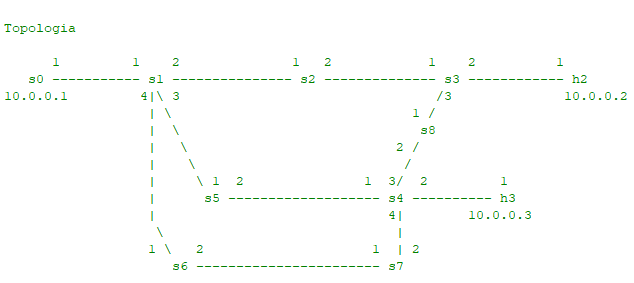
\includegraphics[width=16cm, keepaspectratio]{img/bucle4}
		\caption{Primer escenario con un controlador}
		\label{figura:bucle4}
	\end{figure}
	
	\begin{figure}
		\centering
		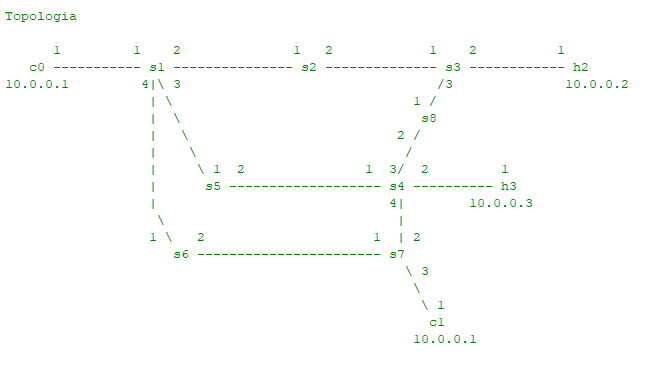
\includegraphics[width=16cm, keepaspectratio]{img/2controllers}
		\caption{Primer escenario con 2 controladores}
		\label{figura:2controllers}
	\end{figure}
	
	Posteriormente, se analizará un escenario mas complejo ~\ref{figura:mesh} y el mismo escenario con 4 controladores en vez de 1 ~\ref{figura:mesh4c}.
	
	\begin{figure}
		\centering
		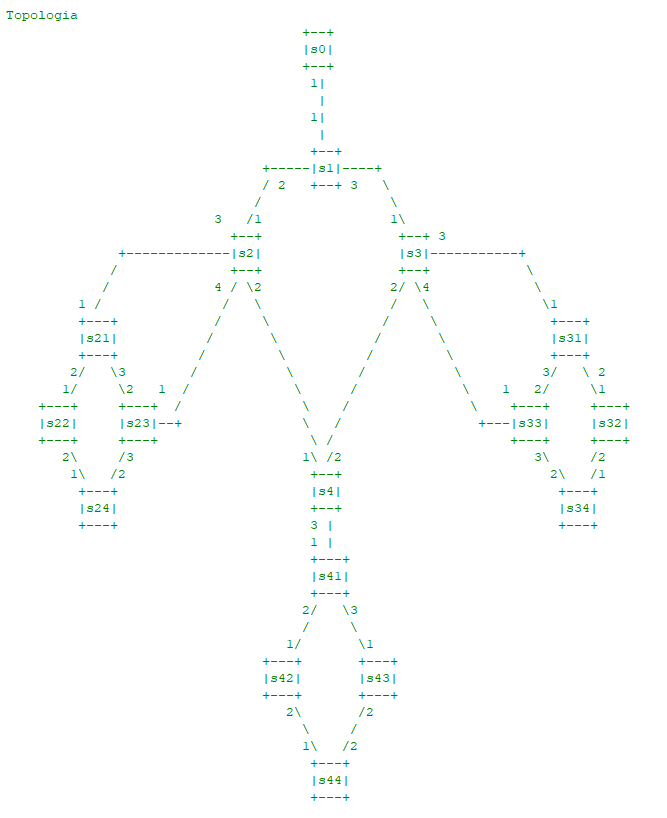
\includegraphics[width=16cm, keepaspectratio]{img/mesh}
		\caption{Segundo escenario con 1 controlador}
		\label{figura:mesh}
	\end{figure}
	
	\begin{figure}
		\centering
		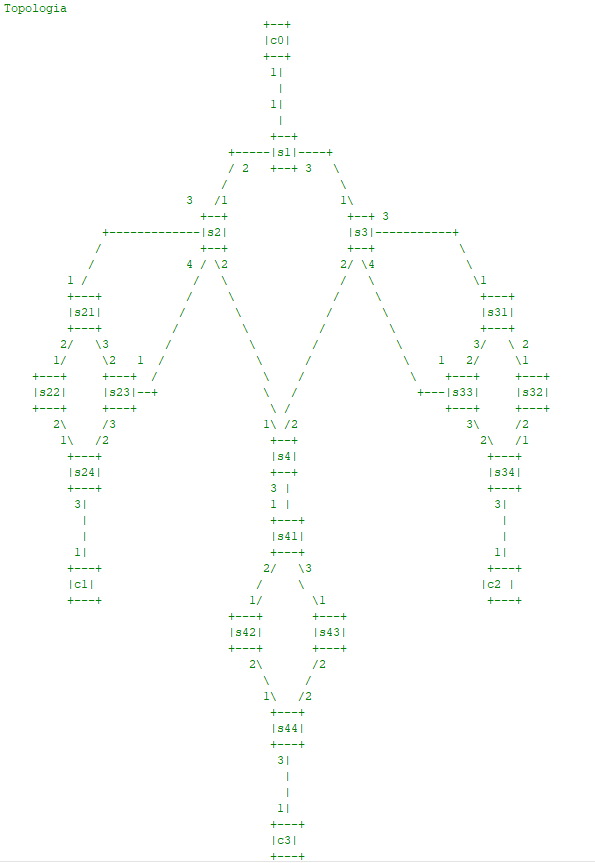
\includegraphics[width=16cm, keepaspectratio]{img/mesh4c}
		\caption{Segundo escenario con 4 controladores}
		\label{figura:mesh4c}
	\end{figure}
	
	\section{Planificación temporal}
	\label{sec:planificacion-temporal}
	
	El trabajo de fin de grado se ha realizado durante mas de un año, de forma intermitente, principalmente en fines de semana y festivos. Durante todo este tiempo, hemos estado intercambiando correos, y teniendo varias reuniones de seguimiento, principalmente porque un requisito importante de este trabajo de fin de grado era entender perfectamente lo que ocurría en el escenario, viendo así capas muchos mas bajas de las que finalmente he tenido que usar para realizar los experimentos.
	Además ha habido varios problemas con las herramientas de trabajo que han ralentizado mucho el trabajo, con periodos de inactividad de varios meses intentando solventar los problemas.
	
	
	%%%%%%%%%%%%%%%%%%%%%%%%%%%%%%%%%%%%%%%%%%%%%%%%%%%%%%%%%%%%%%%%%%%%%%%%%%%%%%%%
	%%%%%%%%%%%%%%%%%%%%%%%%%%%%%%%%%%%%%%%%%%%%%%%%%%%%%%%%%%%%%%%%%%%%%%%%%%%%%%%%
	% ESTADO DEL ARTE %
	%%%%%%%%%%%%%%%%%%%%%%%%%%%%%%%%%%%%%%%%%%%%%%%%%%%%%%%%%%%%%%%%%%%%%%%%%%%%%%%%
	
	\cleardoublepage
	\chapter{Estado del arte}
	\label{chap:estado}
	
	En este capítulo se detallan las tecnologías utilizadas en el desarrollo del proyecto.	
	
	\section{Mininet} 
	\label{sec:seccion1}
	
	Mininet es......
	
	Se ha utilizado para ...
	
	\section{Wireshark} 
	\label{sec:seccion2}
	
	Wireshark es......	
	Se ha utilizado para ...	
	
	\section{Python} 
	\label{sec:seccion3}
	
	\section{Otros} 
	\label{sec:seccion4}
	
	%%%%%%%%%%%%%%%%%%%%%%%%%%%%%%%%%%%%%%%%%%%%%%%%%%%%%%%%%%%%%%%%%%%%%%%%%%%%%%%%
	%%%%%%%%%%%%%%%%%%%%%%%%%%%%%%%%%%%%%%%%%%%%%%%%%%%%%%%%%%%%%%%%%%%%%%%%%%%%%%%%
	% DISEÑO E IMPLEMENTACIÓN %
	%%%%%%%%%%%%%%%%%%%%%%%%%%%%%%%%%%%%%%%%%%%%%%%%%%%%%%%%%%%%%%%%%%%%%%%%%%%%%%%%
	
	\cleardoublepage
	\chapter{Diseño e implementación}
	\label{sec:diseno}
	 
	 No se si aplica.
	
	
	
	%%%%%%%%%%%%%%%%%%%%%%%%%%%%%%%%%%%%%%%%%%%%%%%%%%%%%%%%%%%%%%%%%%%%%%%%%%%%%%%%
	%%%%%%%%%%%%%%%%%%%%%%%%%%%%%%%%%%%%%%%%%%%%%%%%%%%%%%%%%%%%%%%%%%%%%%%%%%%%%%%%
	% EXPERIMENTOS Y VALIDACIÓN %
	%%%%%%%%%%%%%%%%%%%%%%%%%%%%%%%%%%%%%%%%%%%%%%%%%%%%%%%%%%%%%%%%%%%%%%%%%%%%%%%%
	
	\cleardoublepage
	\chapter{Experimentos y validación}
	\label{chap:experimentos}
	
	Como se ha comentado previamente, se va a realizar el experimento con dos esquemas muy diferentes, para ver la diferencia de tener un controlador o varios.
	
	Para el primer caso, el visto en ~\ref{figura:bucle4} y ~\ref{figura:2controllers}. Hemos obtenido los siguientes resultados:
	
	\begin{figure}
		\centering
		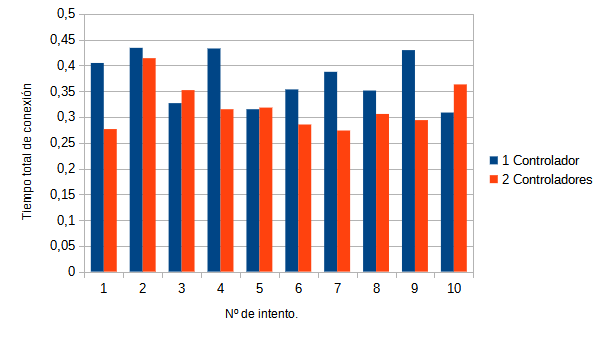
\includegraphics[width=16cm, keepaspectratio]{img/comparativabucle4}
		\caption{Comparativa de tiempos en el primer escenario}
		\label{figura:comparativabucle4}
	\end{figure}
	
	\begin{figure}
		\centering
		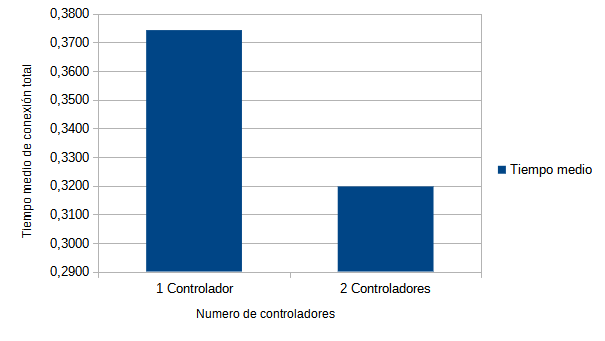
\includegraphics[width=16cm, keepaspectratio]{img/comparativamediasbucle}
		\caption{Comparativa de media de tiempos en el primer escenario}
		\label{figura:mediabucle4}
	\end{figure}
	
	Para el caso de 1 controlador, los esquemas se han ido conectando de las siguientes formas:
	
	\begin{figure}
		\centering
		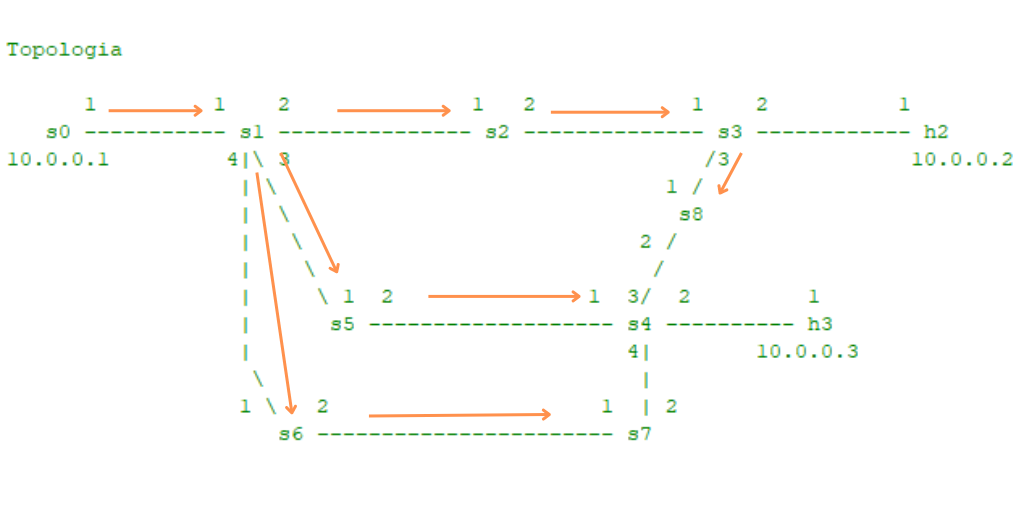
\includegraphics[width=16cm, keepaspectratio]{img/escenario1_1c_1}
		\caption{Orden de conexión de los experimentos 1, 3, 4, 5, 6 ,7, 8, 10}
		\label{figura:escenario1_1c_1}
	\end{figure}
	
	\begin{figure}
		\centering
		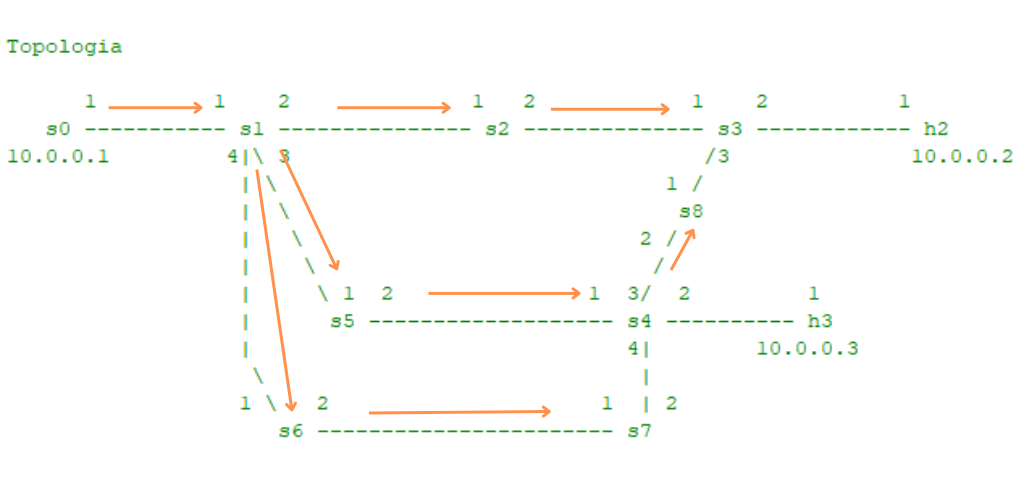
\includegraphics[width=16cm, keepaspectratio]{img/escenario1_1c_2}
		\caption{Orden de conexión de los experimentos 2, 9}
		\label{figura:escenario1_1c_2}
	\end{figure}
	
	Para el caso de 2 controladores, como era de esperar es bastante diferente, quedando así:
	
	\begin{figure}
		\centering
		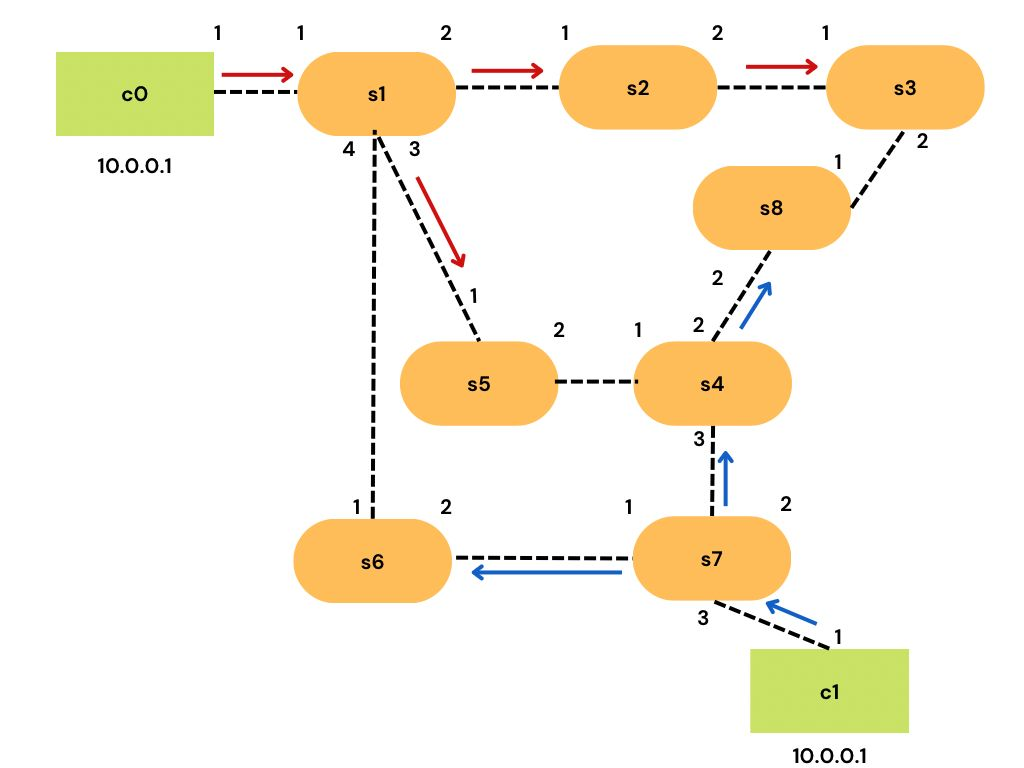
\includegraphics[width=16cm, keepaspectratio]{img/escenario1_2c_1}
		\caption{Orden de conexión de los experimentos 1, 4}
		\label{figura:escenario1_2c_1}
	\end{figure}
	
	\begin{figure}
		\centering
		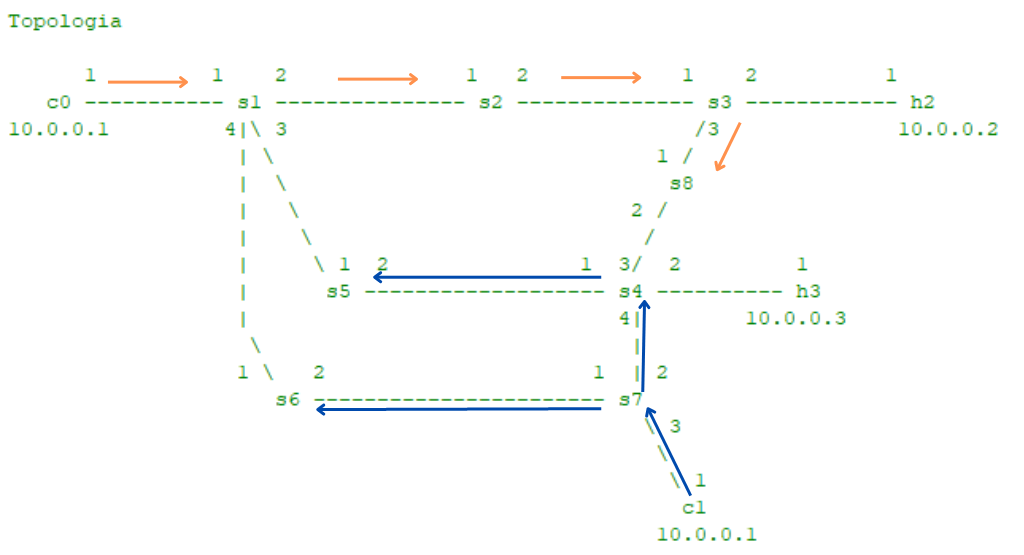
\includegraphics[width=16cm, keepaspectratio]{img/escenario1_2c_2}
		\caption{Orden de conexión de los experimentos 2, 9}
		\label{figura:escenario1_2c_2}
	\end{figure}
	
	\begin{figure}
		\centering
		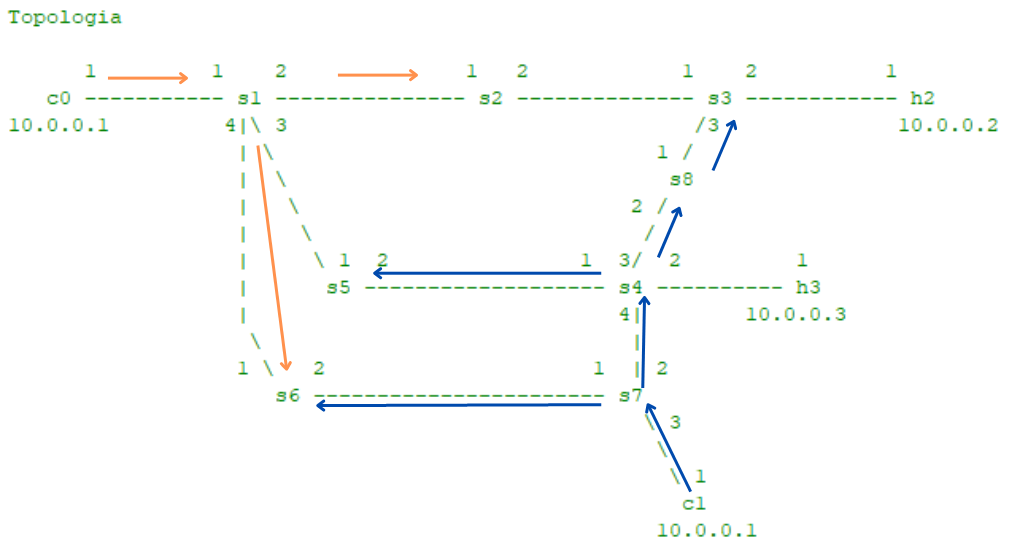
\includegraphics[width=16cm, keepaspectratio]{img/escenario1_2c_3}
		\caption{Orden de conexión del experimento 3}
		\label{figura:escenario_2c_3}
	\end{figure}
	
	\begin{figure}
		\centering
		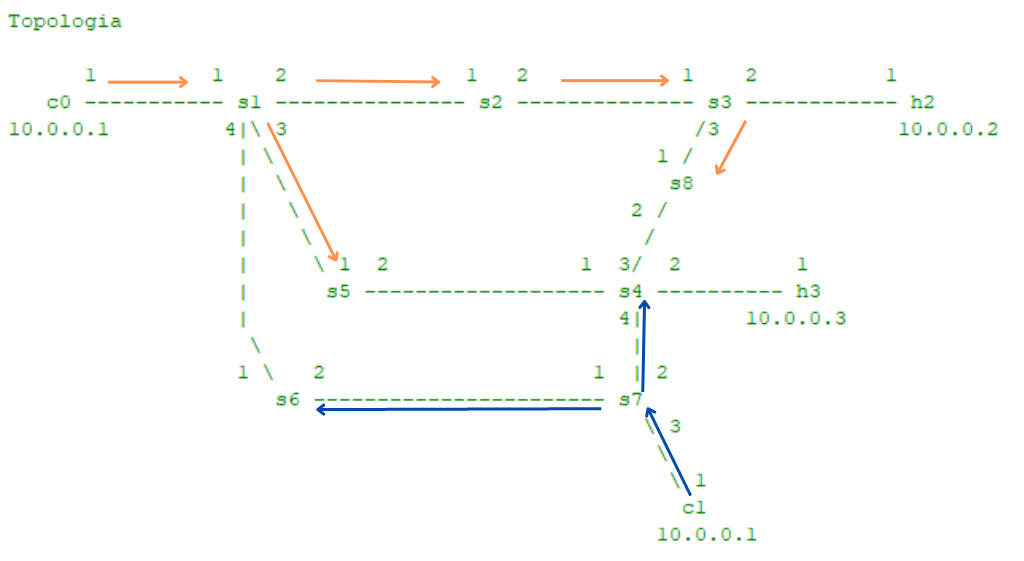
\includegraphics[width=16cm, keepaspectratio]{img/escenario1_2c_4}
		\caption{Orden de conexión del experimento 5}
		\label{figura:escenario1_2c_4}
	\end{figure}
	
	\begin{figure}
		\centering
		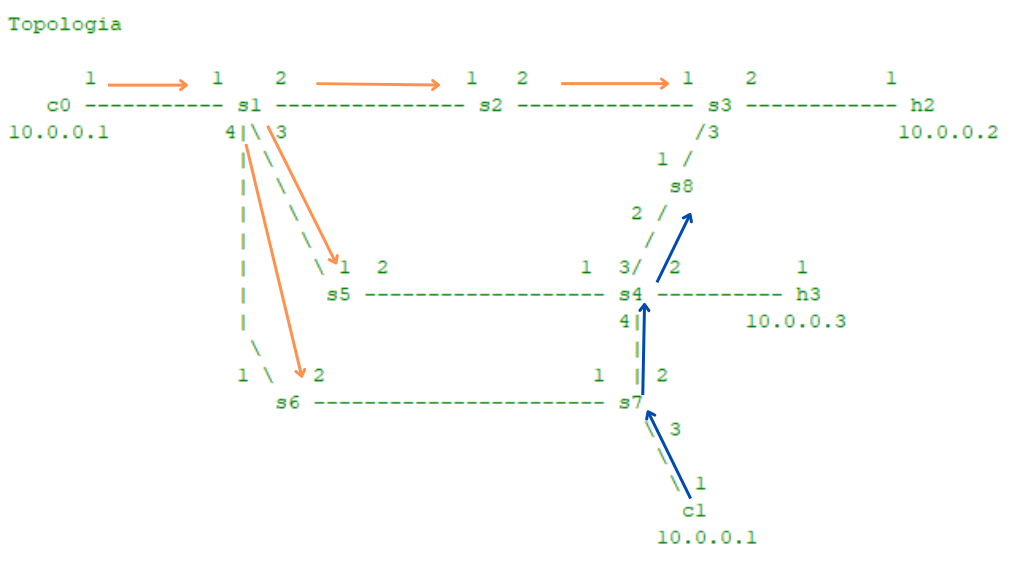
\includegraphics[width=16cm, keepaspectratio]{img/escenario1_2c_5}
		\caption{Orden de conexión del experimento 6}
		\label{figura:escenario1_2c_5}
	\end{figure}
	
	\begin{figure}
		\centering
		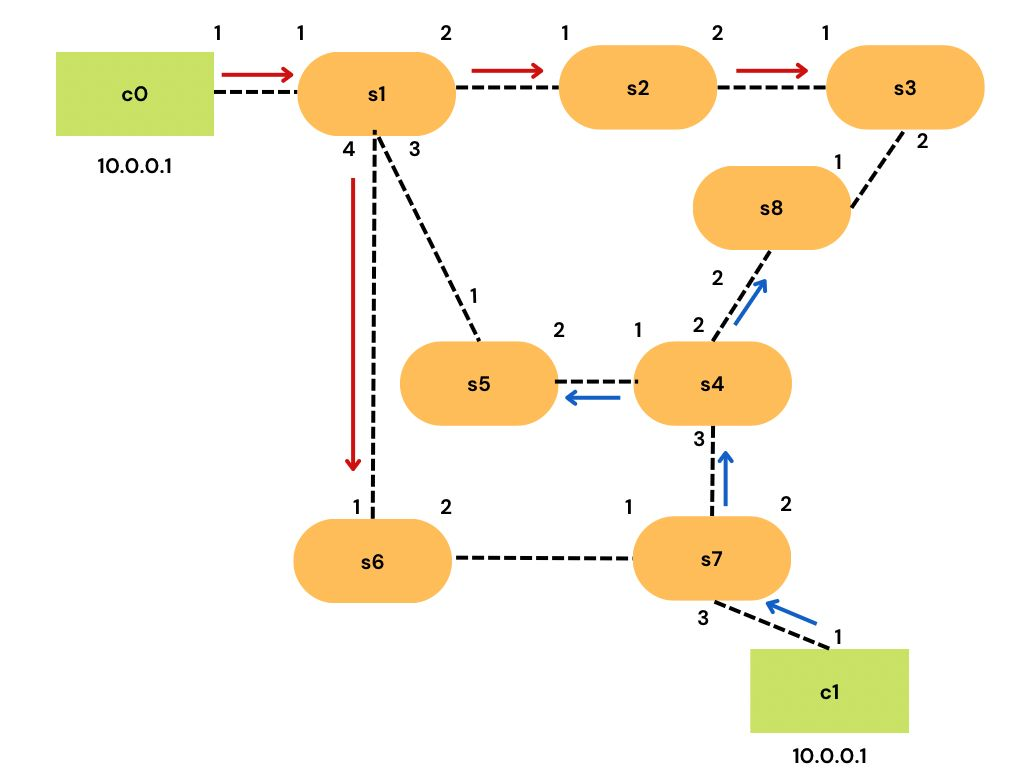
\includegraphics[width=16cm, keepaspectratio]{img/escenario1_2c_6}
		\caption{Orden de conexión del experimento 7}
		\label{figura:escenario1_2c_6}
	\end{figure}
	
	\begin{figure}
		\centering
		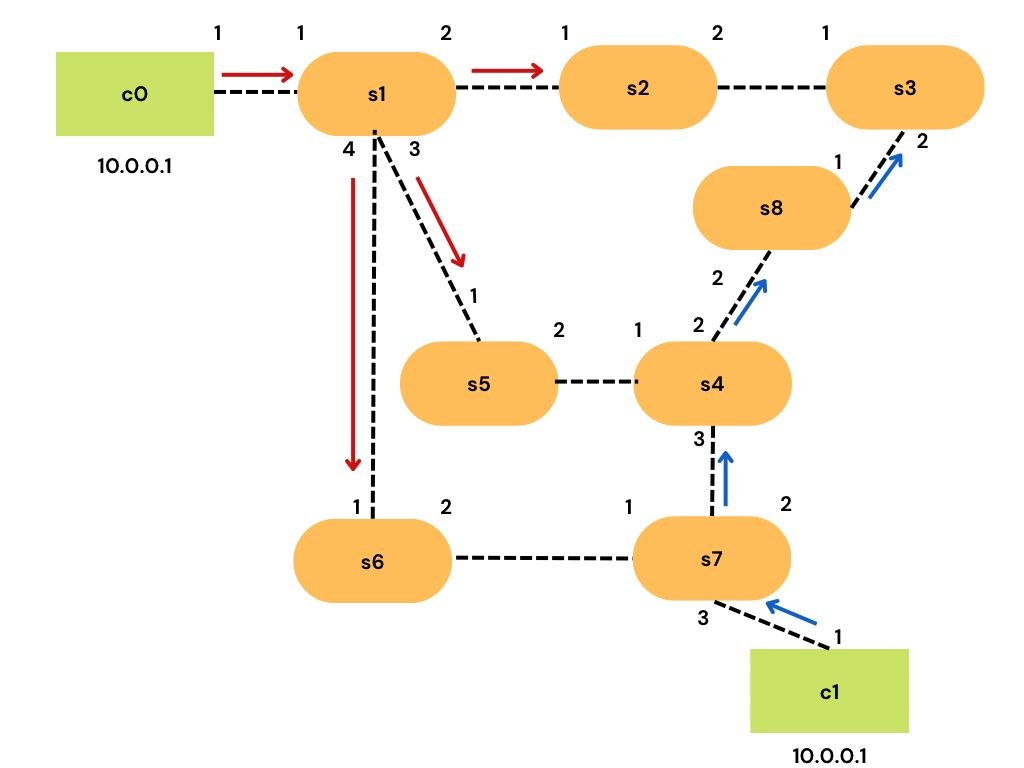
\includegraphics[width=16cm, keepaspectratio]{img/escenario1_2c_7}
		\caption{Orden de conexión del experimento 8}
		\label{figura:escenario1_2c_7}
	\end{figure}
	
		\begin{figure}
		\centering
		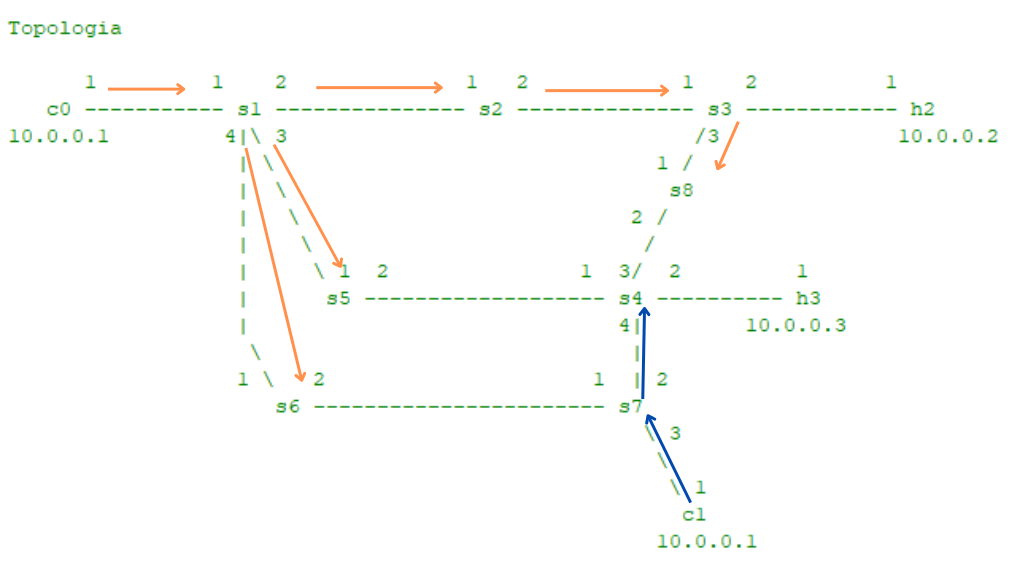
\includegraphics[width=16cm, keepaspectratio]{img/escenario1_2c_8}
		\caption{Orden de conexión del experimento 10}
		\label{figura:escenario1_2c_8}
	\end{figure}

	
	Para el segundo caso, se trabaja con un escenario mucho mas grande, el visto en ~\ref{figura:mesh} y ~\ref{figura:mesh4c}. Hemos obtenido los siguientes resultados:
	
	\begin{figure}
		\centering
		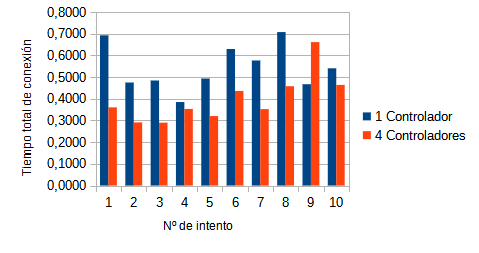
\includegraphics[width=16cm, keepaspectratio]{img/comparativamesh}
		\caption{Comparativa de tiempos en el segundo escenario}
		\label{figura:comparativamesh}
	\end{figure}
	
	\begin{figure}
		\centering
		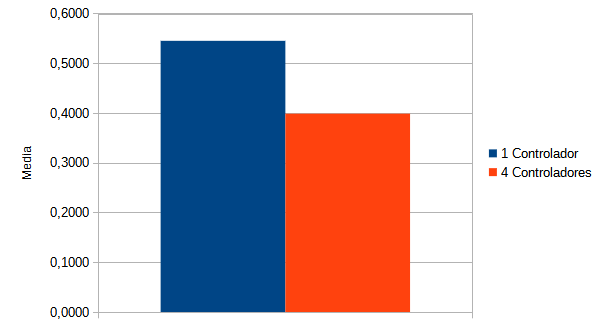
\includegraphics[width=16cm, keepaspectratio]{img/comparativamediamesh}
		\caption{Comparativa de media de tiempos en el segundo escenario}
		\label{figura:mediamesh}
	\end{figure}
	
	%%%%%%%%%%%%%%%%%%%%%%%%%%%%%%%%%%%%%%%%%%%%%%%%%%%%%%%%%%%%%%%%%%%%%%%%%%%%%%%%
	%%%%%%%%%%%%%%%%%%%%%%%%%%%%%%%%%%%%%%%%%%%%%%%%%%%%%%%%%%%%%%%%%%%%%%%%%%%%%%%%
	% RESULTADOS %
	%%%%%%%%%%%%%%%%%%%%%%%%%%%%%%%%%%%%%%%%%%%%%%%%%%%%%%%%%%%%%%%%%%%%%%%%%%%%%%%%
	
	\cleardoublepage
	\chapter{Resultados}
	\label{chap:resultados}
	
 
 	Aqui explicar todos los escenarios, con datos, seguramente sea lo que esta en el apartado anterior.
	
	
	%%%%%%%%%%%%%%%%%%%%%%%%%%%%%%%%%%%%%%%%%%%%%%%%%%%%%%%%%%%%%%%%%%%%%%%%%%%%%%%%
	%%%%%%%%%%%%%%%%%%%%%%%%%%%%%%%%%%%%%%%%%%%%%%%%%%%%%%%%%%%%%%%%%%%%%%%%%%%%%%%%
	% CONCLUSIONES %
	%%%%%%%%%%%%%%%%%%%%%%%%%%%%%%%%%%%%%%%%%%%%%%%%%%%%%%%%%%%%%%%%%%%%%%%%%%%%%%%%
	
	\cleardoublepage
	\chapter{Conclusiones}
	\label{chap:conclusiones}
	
	Explicar las conclusiones sacadas de comparar los escenarios con 1 y varios controladores.
	
	\section{Consecución de objetivos}
	\label{sec:consecucion-objetivos}
	
	Esta sección es la sección espejo de las dos primeras del capítulo de objetivos, donde se planteaba el objetivo general y se elaboraban los específicos.
	
	\section{Aplicación de lo aprendido}
	\label{sec:aplicacion}
	
	\begin{enumerate}
		\item Arquitectura de Redes de Ordenadores
		\item 
	\end{enumerate}
	
	
	\section{Lecciones aprendidas}
	\label{sec:lecciones_aprendidas}
	
	Durante todo el trabajo de fin de grado he ido aprendiendo sobre Openflow, algo que no me ha costado demasiado ya que trabajo en el sector del tráfico ferroviario y es bastante similar la casuística que se daba aquí.
	
	\begin{enumerate}
		\item Durante todo el trabajo de fin de grado he ido aprendiendo sobre Openflow, algo que no me ha costado demasiado ya que trabajo en el sector del tráfico ferroviario y es bastante similar la casuística que se daba aquí.
		\item LaTeX, ya que la memoria se ha realizado íntegramente con LaTeX.
		\item Python. Pese a que el trabajo en si no tenía programación, he tenido que aprender las bases del lenguaje para entender que hacían los scripts.
	\end{enumerate}
	
	
	\section{Trabajos futuros}
	\label{sec:trabajos_futuros}
	
	Visto lo aprendido y analizado en este trabajo de fin de grado, creo que sería una opción a tener en cuenta el optimizar los circuitos del sistema, creando algo de lógica en los controladores si fuese posible. **
	
	
	%%%%%%%%%%%%%%%%%%%%%%%%%%%%%%%%%%%%%%%%%%%%%%%%%%%%%%%%%%%%%%%%%%%%%%%%%%%%%%%%
	%%%%%%%%%%%%%%%%%%%%%%%%%%%%%%%%%%%%%%%%%%%%%%%%%%%%%%%%%%%%%%%%%%%%%%%%%%%%%%%%
	% APÉNDICE(S) %
	%%%%%%%%%%%%%%%%%%%%%%%%%%%%%%%%%%%%%%%%%%%%%%%%%%%%%%%%%%%%%%%%%%%%%%%%%%%%%%%%
	
	\cleardoublepage
	
	%%%%%%%%%%%%%%%%%%%%%%%%%%%%%%%%%%%%%%%%%%%%%%%%%%%%%%%%%%%%%%%%%%%%%%%%%%%%%%%%
	%%%%%%%%%%%%%%%%%%%%%%%%%%%%%%%%%%%%%%%%%%%%%%%%%%%%%%%%%%%%%%%%%%%%%%%%%%%%%%%%
	% BIBLIOGRAFIA %
	%%%%%%%%%%%%%%%%%%%%%%%%%%%%%%%%%%%%%%%%%%%%%%%%%%%%%%%%%%%%%%%%%%%%%%%%%%%%%%%%
	
	\cleardoublepage
	
	% Las siguientes dos instrucciones es todo lo que necesitas
	% para incluir las citas en la memoria
	\bibliographystyle{abbrv}
	\bibliography{memoria}  % memoria.bib es el nombre del fichero que contiene
	% las referencias bibliográficas. Abre ese fichero y mira el formato que tiene,
	% que se conoce como BibTeX. Hay muchos sitios que exportan referencias en
	% formato BibTeX. Prueba a buscar en http://scholar.google.com por referencias
	% y verás que lo puedes hacer de manera sencilla.
	% Más información: 
	% http://texblog.org/2014/04/22/using-google-scholar-to-download-bibtex-citations/
	
\end{document}
